%%%%%%%%%%%%%%%%%%%%%%%%%%%%%%%%%%%%%%%%%%%%%%%%%%%%%%%%%%%%%%%%%%%%%%%%%%%%%%%%%%
\begin{frame}[fragile]\frametitle{}
\begin{center}
{\Large Descriptive Statistics - Expected Value way}
\end{center}
\end{frame}


%%%%%%%%%%%%%%%%%%%%%%%%%%%%%%%%%%%%%%%%%%%%%%%%%%%%%%%%%%
\begin{frame}[fragile]\frametitle{Expected Value: Investment Decision}	
\begin{itemize}
\item Weights as probabilities
\item Evaluate which investment option is better
\item Weights, being probabilities, sum up to ??
\end{itemize}
\begin{center}
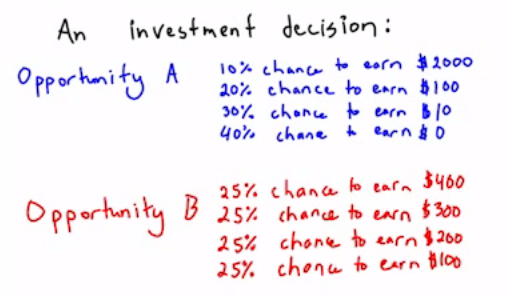
\includegraphics[width=0.75\linewidth,keepaspectratio]{probavrg}
\end{center}
Answer?
\end{frame}


%%%%%%%%%%%%%%%%%%%%%%%%%%%%%%%%%%%%%%%%%%%%%%%%%%%%%%%%%%
\begin{frame}
\frametitle{Expected Value}

\begin{definition}[Expected Value]
\textbf{Expected Value} is the average gain or loss of an event if the procedure is repeated many times.  We can compute the expected value by multiplying each outcome by the probability of that outcome, then adding up the products.
\end{definition}

\begin{center}
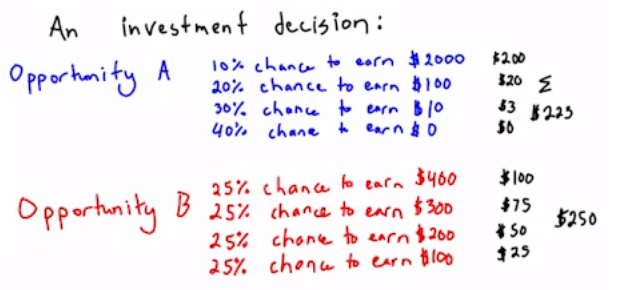
\includegraphics[width=0.75\linewidth,keepaspectratio]{probavrg1}
\end{center}
\end{frame}


%%%%%%%%%%%%%%%%%%%%%%%%%%%%%%%%%%%%%%%%%%%%%%%%%%%%%%%%%%
\begin{frame}
\frametitle{Expected value: The Mean}

The most common way to define the location of a distribution is as the
{\bf expected value}.

If $X$ is a discrete random variable with sample space $x_1, x_2,
\ldots$, the expected value is

\begin{eqnarray*}
EX &=& x_1\cdot P(X=x_1) + x_2\cdot P(X=x_2) + \cdots\\ &=& \sum_i x_i
\cdot P(X=x_i).
\end{eqnarray*}

If $X$ is a continuous random variable, the definition of $EX$
requires integral calculus, so we will not give it here (but it is
analogous).

\end{frame}

%%%%%%%%%%%%%%%%%%%%%%%%%%%%%%%%%%%%%%%%%%%%%%%%%%%%%%%%%%
\begin{frame}
\frametitle{Expected value}

Suppose we are interested in the number of times a Michigan resident
has visited Florida, denoted $X$, as described by the following
distribution:

\begin{center}
\begin{tabular}{lllllllll}
$x$         & 0   & 1 & 2 & 3 & 4 & 5 & 6\\\hline
$P(X=x)$    & 0.3 & 0.1 & 0.2 & 0.1 & 0.06 & 0.08 & 0.16\\
$P(X\le x)$ & 0.3 & 0.4 & 0.6 & 0.7 & 0.76 & 0.84 & 1\\\hline
\end{tabular}
\end{center}

The expected value of $X$ is

\begin{eqnarray*}
EX &=& 0\times 0.3 + 1\times 0.1 + 2\times 0.2 + 3\times 0.1 +
4\times 0.06 +\\&& 5\times 0.08 + 6\times 0.16\\
&=& 2.4
\end{eqnarray*}

\end{frame}

%%%%%%%%%%%%%%%%%%%%%%%%%%%%%%%%%%%%%%%%%%%%%%%%%%%%%%%%%%
\begin{frame}
\frametitle{Expected value}

The expected value is the balancing point if we weight each point in
the sample space by its probability:

\begin{center}
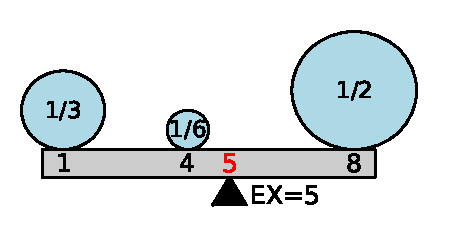
\includegraphics{035.pdf}
\end{center}

This distribution in tabular form:

\begin{center}
\begin{tabular}{llll}\hline
x      & 1 & 4 & 8\\
P(X=x) & 1/3 & 1/6 & 1/2\\\hline
\end{tabular}
\end{center}

\end{frame}

%%%%%%%%%%%%%%%%%%%%%%%%%%%%%%%%%%%%%%%%%%%%%%%%%%%%%%%%%%%
%\begin{frame}
%\frametitle{Expected values of functions of random variables}
%
%Suppose we have a function $f(x)$, and random variable $X$.  By taking
%$f(X)$ we get a new random variable, with its own distribution and
%expected value.  
%
%For discrete random variables, the expected value of $f(X)$ is
%calculated as
%
%$$
%Ef(X) = \sum_i f(x_i)\cdot P(X=x_i),
%$$
%
%where the sum runs over the sample space of $X$.
%
%\end{frame}

%%%%%%%%%%%%%%%%%%%%%%%%%%%%%%%%%%%%%%%%%%%%%%%%%%%%%%%%%%
\begin{frame}
\frametitle{Expected values of functions of random variables}

For example,

\begin{center}
\begin{tabular}{cll}
{$x$} & {$P(X=x)$}\\\hline 
-1 & \hspace{0.8cm}0.2\\
 0 & \hspace{0.8cm}0.4\\
 1 & \hspace{0.8cm}0.4\\\hline
\end{tabular}
\end{center}

The expected values of some functions of $X$ are:

$$
\begin{array}{ccccc}
EX &=& -1\cdot 0.2 + 0\cdot 0.4 + 1\cdot 0.4 &=& 0.2\\
EX^2 &=& (-1)^2\cdot 0.2 + 0^2\cdot 0.4 + 1^2\cdot 0.4 &=& 0.6\\
E1/(2+X) &=& 1\cdot 0.2 + (1/2)\cdot 0.4 + (1/3)\cdot 0.4 &\approx& 0.53  
\end{array}
$$

\end{frame}

%%%%%%%%%%%%%%%%%%%%%%%%%%%%%%%%%%%%%%%%%%%%%%%%%%%%%%%%%%%
%\begin{frame}
%\frametitle{Expected values of functions of random variables}
%
%In general, the expected value of $f(X)$ is not the same as applying
%$f$ to the expected value of $X$ (i.e.\ $f(EX) \ne Ef(X)$).
%
%\textcolor{blue}{\bf Example:} Suppose we have a population in which
%$1/3$ of the people are 160cm tall, $1/3$ of the people are 170cm
%tall, and $1/3$ of the people are 180cm tall.
%
%The expected height is $160/3 + 170/3 + 180/3 = 170$.
%
%The expected squared height is $160^2/3 + 170^2/3 + 180^2/3 \approx
%28967$.
%
%But the square of the expected height is $170^2 = 28900$.
%
%\end{frame}
%
%
%\begin{frame}
%\frametitle{Expected values of functions of random variables}
%
%\textcolor{blue}{\bf Example:} Suppose we are interested in 5 cars
%that have given miles per gallon (MPG) values, and that are driven by
%given fractions of the population (assume for simplicity that these
%are the only 5 car types available):
%
%\begin{center}
%\begin{tabular}{llllll}\\\hline
%MPG & 22 & 24 & 28 & 29 & 35\\
%Frequency & 0.3 & 0.1 & 0.2 & 0.1 & 0.3\\\hline
%\end{tabular}
%\end{center}
%
%The expected MPG is
%
%$$
%22\times 0.3 + 24\times 0.1 + 28\times 0.2 + 29\times 0.1 + 35\times 0.3 = 28.
%$$
%
%If we are interested in gallons per mile (GPM), the expected value is
%
%$$ (1/22)\times 0.3 + (1/24)\times 0.1 + (1/28)\times 0.2 +
%(1/29)\times 0.1 + (1/35)\times 0.3 \approx 0.037.
%$$
%
%\end{frame}
%
%
%
%\begin{frame}
%\frametitle{Properties of the expected value}
%
%\begin{itemize}
%
%\item The expected value of a constant is just the value of the
%  constant.  For example, if $X$ is a random variable that always
%  takes on the value $7$, then the distribution of $X$ is $P(X=7)=1$,
%  so the expected value is $7\times P(X=7) = 7\times 1 = 7$.
%
%\item The expected value is \textcolor{purple}{linear}, which means
%  that if we have constants $a$ and $b$ and a random variable $X$,
%  then
%
%$$
%E(a+bX) = a + bEX.
%$$
%
%\item The expected value is \textcolor{purple}{additive}: if $X$ and
%  $Y$ are two random variables, then $E(X+Y) = EX + EY$.
%
%\end{itemize}
%
%\end{frame}
%
%\begin{frame}
%\frametitle{Properties of the expected value (continued)}
%
%\textcolor{blue}{\bf Example (linearity):} Suppose the sample space is
%$\{-1,1\}$ and $P(X=-1)=0.3$, $P(X=1) = 0.7$.  
%
%By direct calculation, $EX = -1\cdot 0.3 + 1\cdot 0.7 = 0.4$.  
%
%If we define $Y = 3 - 2X$ then the sample space of $Y$ is $\{1,5\}$,
%and the probabilities are $P(Y=1) = P(X=1) = 0.7$, $P(Y=5) = P(X=-1) =
%0.3$.  
%
%So again by direct calculation, $EY = 1\cdot 0.7 + 5\cdot 0.3 = 2.2$.
%
%Alternatively, we can use the linearity property, $EY = 3 - 2\cdot EX
%= 3 - 2\cdot 0.4 = 2.2$.
%
%\end{frame}
%
%\begin{frame}
%\frametitle{Properties of the expected value (continued)}
%
%\textcolor{blue}{\bf Example (additivity):} suppose $X$ and $Y$ are
%independent and both have sample space $\{-1,1\}$ with probability
%$0.5$ of taking either value.  
%
%By direct calculation, $EX=EY=0$.
%
%If $Z=X+Y$, the sample space of $Z$ is $\{-2,0,2\}$ with probabilities
%$P(Z=-2) = P(X=-1\;{\rm and}\;Y=-1) = 1/4$,
%$P(Z=2) = P(X=1\;{\rm and}\;Y=1) = 1/4$, and therefore $P(Z=0) =
%1/2$.
%
%So again by direct calculation, $EZ = -2\cdot 0.25 + 0\cdot 0.5 +
%2\cdot 0.25 = 0$.  
%
%Alternatively, we can use the additivity property, $EZ = EX+EY = 0+0 =
%0$.
%
%\end{frame}
%
%
%\begin{frame}
%\frametitle{Properties of the expected value (continued)}
%
%\textcolor{purple}{Comment:} The linearity and additivity properties
%may seem obvious, or automatic -- but they are not.
%
%Many statistics we will use later like the median and variance do not
%satisfy one or both of these properties.
%
%\end{frame}
%
%
%\begin{frame}
%\frametitle{Properties of the expected value (continued)}
%
%A consequence of linearity is that the expected value behaves
%naturally when we change the measurement units.
%
%\textcolor{blue}{\bf Example:} Suppose we measure five peoples'
%heights in inches:
%
%$$
%72,\, 68,\, 73,\, 65,\, 69
%$$
%
%The mean height is 69.4 inches.  One inch equals 2.54 centimeters, so
%the equivalent heights in centimeters are
%
%$$
%182.88,\, 172.72,\, 185.42,\, 165.10,\, 175.26.
%$$
%
%The mean height in centimeters is 176.28cm.  If we simply convert the
%mean height in inches to centimeters we get 69.4$\times$2.54 =
%176.28cm, the same value.
%
%\end{frame}
%
%
%\begin{frame}
%\frametitle{Mean squared difference}
%
%For an arbitrary constant value $\theta$, the quantity
%
%\begin{center}
%$E(X-\theta)^2$
%\end{center}
%
%measures the \textcolor{purple}{mean squared difference} between $X$
%and $\theta$.
%
%\begin{center}
%\scalebox{0.4}{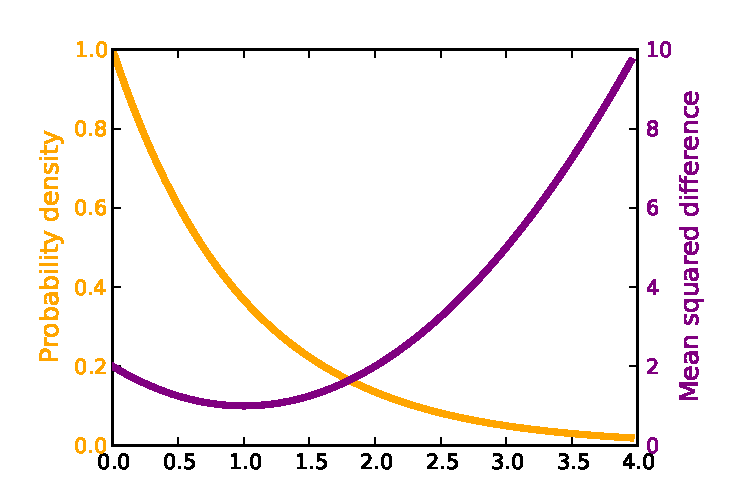
\includegraphics{041.pdf}}
%\end{center}
%
%It is a fact that setting $\theta = EX$ gives the smallest possible
%value for $E(X-\theta)^2$.  Note that $EX=1$ in the graph.
%
%\end{frame}
%
%
%\begin{frame}
%\frametitle{Mean squared difference}
%
%\textcolor{blue}{\bf Example:} Suppose $X$ is a ``Bernoulli'' random
%variable, meaning it can take on only two values: $P(X=1)=p$ and
%$P(X=0)=1-p$.  
%
%The expected value of a Bernoulli trial is 
%
%$$1\cdot P(X=1) + 0\cdot P(X=0) = 1\cdot p + 0\cdot (1-p) = p.$$  
%
%The value of $E(X-\theta)^2$ is
%
%\begin{eqnarray*}
%\lefteqn{(1-\theta)^2\cdot P(X=1) + (0-\theta)^2\cdot P(X=0)}\\ &=&
%(1-\theta)^2p + (0-\theta)^2(1-p)\\ &=& \theta^2 - 2p\theta+ p.\\
%\end{eqnarray*}
%
%\vspace{-0.5cm}
%
%We want to minimize this as a function of $\theta$, so differentiate
%with respect to $\theta$ to get $2\theta - 2p=0$, then solve to get
%$\theta=p = EX$.
%
%\end{frame}
%
%
%\begin{frame}
%\frametitle{Exercises}
%
%\begin{enumerate}
%
%\item For the following distribution, what are $EX$, $EX^2$,
%  $\sqrt{EX^2}$ and $(EX)^2$?
%
%\begin{center}
%\begin{tabular}{llllll}\\\hline
%$x$      & -2 & 0 & 2 \\
%$P(X=x)$ & 0.2 & 0.5 & 0.3 \\\hline
%\end{tabular}
%\end{center}
%
%\item Complete the following distribution to give the lowest possible
%  value for $EX$.
%
%\begin{center}
%\begin{tabular}{llllll}\\\hline
%$x$      & -2 & 0 & 2 \\
%$P(X=x)$ & 0.2 & ? & ? \\\hline
%\end{tabular}
%\end{center}
%
%\item Compute the expected values of the following three
%  distributions, and explain how they are related.
%
%\begin{center}
%\begin{tabular}{l|lll|lll|lll}
%\multicolumn{1}{c}{}&\multicolumn{3}{c}{Distribution 1} &
%\multicolumn{3}{c}{Distribution 2} &
%\multicolumn{3}{c}{Distribution 3}\\\hline 
%$x$      & -2  & 0   & 2   & -4  & 0   & 4   & -1  & 1   & 3 \\
%$P(X=x)$ & 0.2 & 0.5 & 0.3 & 0.2 & 0.5 & 0.3 & 0.2 & 0.5 & 0.3 \\\hline
%\end{tabular}
%\end{center}
%
%\end{enumerate}
%
%\end{frame}
%
%\begin{frame}
%\frametitle{Solutions}
%
%\begin{enumerate}
%
%\item 
%
%\item You want to put the missing probability on the lowest possible
%  value, so you should put all the remaining probability (0.8 units)
%  on x=0, giving a mean value of -0.4.
%
%\item Let X follow distribution 1, Y follow distribution 2, and Z
%  follow distribution 3.  Then the distribution of Y equals the
%  distribution of 2*X, and the distribution of Z equals the
%  distribution of X+1.  Therefore by the linearity property EY=2EX and
%  EZ=EX+1.
%
%\end{enumerate}
%
%\end{frame}
%
%
%

%%%%%%%%%%%%%%%%%%%%%%%%%%%%%%%%%%%%%%%%%%%%%%%%%%%%%%%%%%%
\begin{frame}
\frametitle{Variance}

For a random variable $X$, the quantity $d = X-EX$ is the {\bf
  deviation from the mean}.

The quantity $d^2 = (X-EX)^2$ is the {\bf squared deviation from the
  mean.}

\textcolor{blue}{\bf Example:} If a specific 24 year-old male is
$180$cm tall and the population mean of all 24 year-old males is
$177$cm tall, then this person's deviation from the mean is $d=+3$cm,
and his squared deviation from the mean is $d^2=9{\rm
  cm}^2$.

\end{frame}

%%%%%%%%%%%%%%%%%%%%%%%%%%%%%%%%%%%%%%%%%%%%%%%%%%%%%%%%%%%
\begin{frame}
\frametitle{Variance}

The {\bf variance} of a random variable is $E(X-EX)^2$ -- the expected
squared deviation from the mean.

For example, suppose a random variable has the probability mass function
tabulated below.

\begin{center}
\begin{tabular}{llll}\\\hline
$x$ & -1 & 0 & 1\\
$P(X=x)$ & 0.2 & 0.4 & 0.4\\\hline
\end{tabular}
\end{center}

\end{frame}

%%%%%%%%%%%%%%%%%%%%%%%%%%%%%%%%%%%%%%%%%%%%%%%%%%%%%%%%%%%
\begin{frame}
\frametitle{Variance}

The expected value is 0.2, and the deviations from the mean (and their
squares) are

\begin{center}
\begin{tabular}{llll}\\\hline
$x$ & -1 & 0 & 1\\
$d$ & -1.2 & -0.2 & 0.8\\
$d^2$ & 1.44 & 0.04 & 0.64\\\hline
\end{tabular}
\end{center}

The variance is the expected value of $d^2$:
$$
0.2\cdot 1.44 + 0.4\cdot 0.04 + 0.4\cdot 0.64 = 0.56.
$$

\end{frame}


%%%%%%%%%%%%%%%%%%%%%%%%%%%%%%%%%%%%%%%%%%%%%%%%%%%%%%%%%%%
\begin{frame}
\frametitle{Variance}

Here are two important facts about the variance:

\begin{itemize}

\item The expected value of the deviations from the mean $d$ (or
  equivalently, the centered data), is always exactly zero.  For
  example,

$$
0.2\cdot -1.2 + 0.4\cdot -0.2 + 0.4\cdot 0.8 = 0.
$$

\item The {\bf standard deviation} is the square root of the variance.
  The standard deviation here is $\sqrt{0.56} \approx
  0.75$.

\end{itemize}

\end{frame}

%%%%%%%%%%%%%%%%%%%%%%%%%%%%%%%%%%%%%%%%%%%%%%%%%%%%%%%%%%%%
%\begin{frame}
%\frametitle{Variance}
%
%Let's break down the variance for this distribution:
%
%\begin{center}
%\begin{tabular}{llll}\\\hline
%$x$ & -1 & 0 & 1\\
%$P(X=x)$ & 0.2 & 0.4 & 0.4\\\hline
%\end{tabular}
%\end{center}
%
%The deviations from the mean and their squares are shown in this
%diagram:
%
%\begin{center}
%\scalebox{0.8}{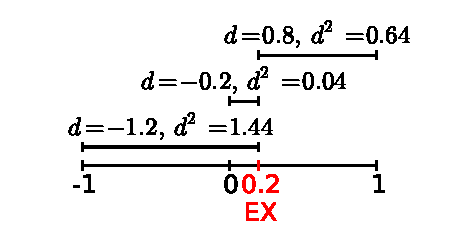
\includegraphics{036.pdf}}
%\end{center}
%
%The variance is
%
%$$
%1.44\times 0.2 + 0.04\times 0.4 + 0.64\times 0.4 = 0.56.
%$$
%
%\end{frame}
%
%
%\begin{frame}
%\frametitle{Properties of the variance and standard deviation}
%
%\begin{itemize}
%
%\item Constants have zero variance and zero standard deviation.
%
%\item Shifting a random variable $X$ by a constant $c$ does not change
%the variance or standard deviation: ${\rm var}(X+c) = {\rm var}(X)$,
%${\rm SD}(X+c) = {\rm SD}(X)$.
%
%\item Scaling affects the variance and standard deviation as follows:
%  ${\rm var}(c\cdot X) = c^2 {\rm var}(X)$, ${\rm SD}(c\cdot X) =
%  |c|{\rm SD}(X)$.
%
%\item If $X$ is measured in some unit, say centimeters, the standard
%deviation of $X$ also has centimeters as units, and the variance of
%$X$ has centimeters$^2$ as units.
%
%\item If $X$ and $Y$ are independent random variables, then ${\rm
%var}(X+Y) = {\rm var}(X) + {\rm var}(Y)$.
%
%\item ${\rm var}(X) = E(X^2) - (EX)^2$ -- this isn't very
%  interpretable, but often is very useful for calculation purposes.
%
%\end{itemize}
%
%\end{frame}
%
%
%\begin{frame}
%\frametitle{Variance and shifting}
%
%\textcolor{purple}{Notation:} The conventional notations for expected
%value and standard deviation are the Greek letters $\mu$ and $\sigma$.
%
%Shifting (or translation) is what happens when we change the origin of
%our scale by adding a constant to each value.  This does not change
%the variance.
%
%The left, below, show the distribution of a random variable $X$, and
%the right shows the distribution of $Y=X+3$.
%
%
%\begin{center}
%\begin{tabular}{cc}
%\scalebox{0.4}{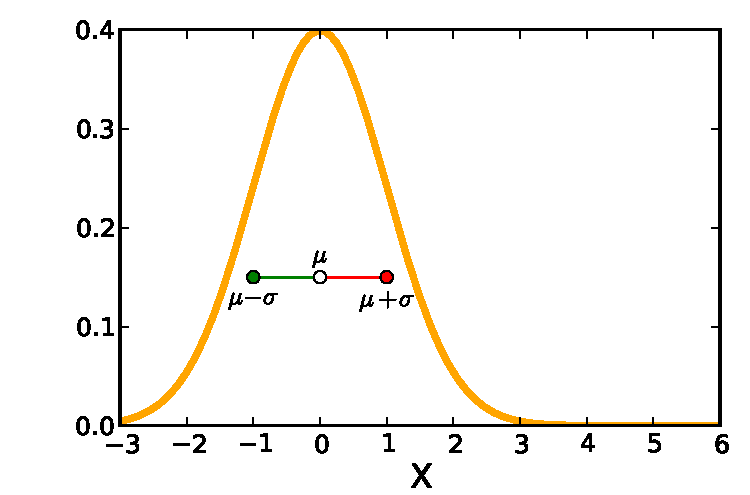
\includegraphics{044-1.pdf}} &
%\scalebox{0.4}{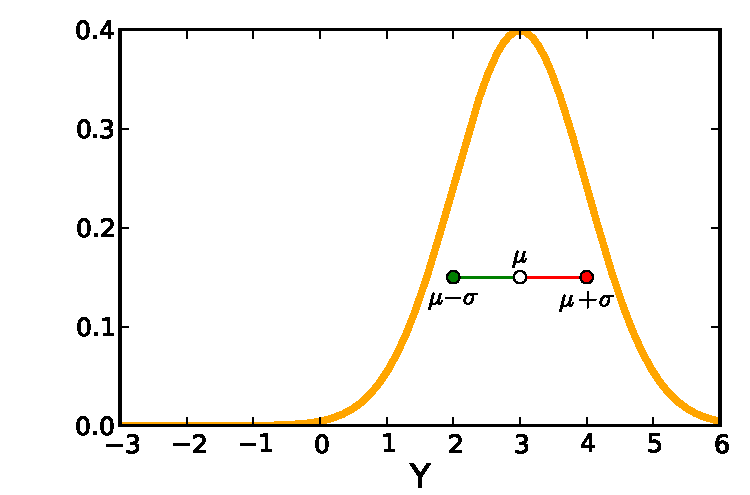
\includegraphics{044-2.pdf}}
%\end{tabular}
%\end{center}
%
%
%\end{frame}
%
%
%
%\begin{frame}
%\frametitle{Variances and distributions}
%
%We have seen that if the data are scaled by a constant $f>0$, then
%both the expected value and the standard deviation are also scaled by
%$f$.  
%
%Thus, the expected value, and deviations from the expected value, have
%fixed relationships to the distribution when the scale changes:
%
%\begin{center}
%\begin{tabular}{cc}
%\scalebox{0.4}{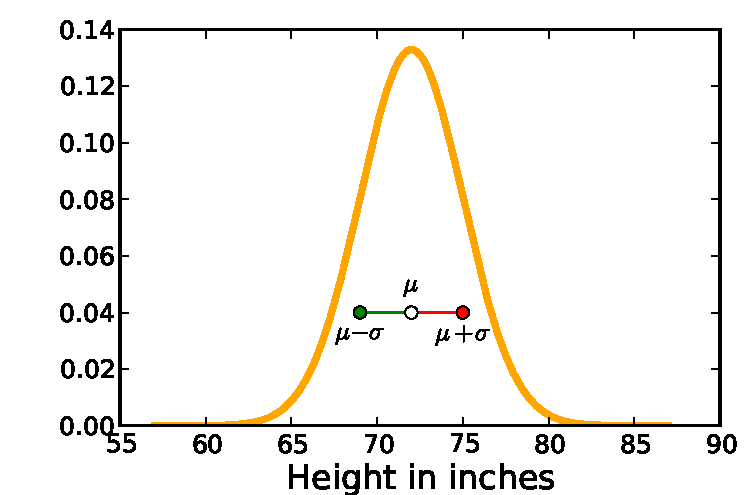
\includegraphics{043-1.pdf}}&
%\scalebox{0.4}{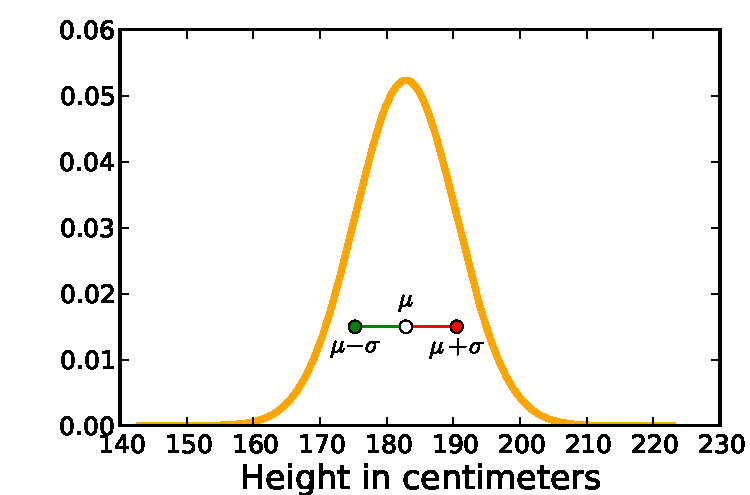
\includegraphics{043-2.pdf}}\\
%\end{tabular}
%\end{center}
%
%On the left $\mu=72, \sigma=3$; on the right $\mu=72\cdot 2.54 =
%182.88$, $\sigma = 3\cdot 2.54 =7.62$.
%
%\end{frame}
%
%
%\begin{frame}
%\frametitle{Exercises}
%
%\begin{enumerate}
%
%\item Suppose the expected height of a population of men is 5'10''
%  with standard deviation 2.1 inches.  If we want to report the
%  expected value, standard deviation, and variance of the heights in
%  centimeters (where 1 inch equals 2.54 centimeters), what would their
%  values be?
%
%\item Suppose two judges are independently rating dance performances
%  on a scale of 1 to 100.  The standard deviation of the first judge's
%  scores is 10, and the standard deviation of the second judge's
%  scores is 12.  If the final score for each dancer is the sum of the
%  two judges' scores, what is the standard deviation of the final
%  scores?
%
%\item Continuing with the previous exercise, what if the average of
%  the two judges' scores is used as the final score instead of the
%  sum.  What is the standard deviation of the final
%  scores?
%
%\end{enumerate}
%
%
%\end{frame}
%
%
%\begin{frame}
%\frametitle{Solutions}
%
%\begin{enumerate}
%
%\item The expected height is 70 inches.  By linearity, the expected
%  value and standard deviation of the height measured in centimeters
%  are 2.54*70 = 177.8 and 2.54*2.1 = 5.3.  The variance in inches is
%  2.1**2 = 4.41, and to convert this to centimeters we scale by
%  2.54**2 = 6.45.  So the variance in centimeters is 4.41*6.45 = 28.4.
%  Note that (up to rounding errors) this equals 5.3**2.
%
%\item The judges are independent, so the variances add: var(Z) =
%  var(X) + var(Y), where X and Y are the two judges' scores, and Z is
%  the total score.  Since the standard deviation is the square-root of
%  the variance, SD(Z) = sqrt(var(X)+var(Y)) = sqrt(10**2+12**2) =
%  sqrt(100+144) = sqrt(244) = 15.6.  Note that you cannot simply sum
%  the two standard deviations.  Also note that the standard deviation
%  of the sum is greater than the standard deviation of either summand.
%  This will always be true if the summands are independent.
%
%\item Here we have to combine the additivity and linearity properties.
%  The average is A = (X+Y)/2, and we know that var(A) = var((X+Y)/2) =
%  var(X+Y)/4.  Thus SD(A) = SD(X+Y)/2 = 15.6/2 = 7.8.
%
%\end{enumerate}
%
%
%\end{frame}
%
%\begin{frame}
%\frametitle{Centering and standardization}
%
%If $X$ is a random variable with mean $\mu$ and variance $\sigma^2$, then
%
%$$
%Y \equiv X-\mu
%$$
%
%is a new random variable with mean 0 and variance $\sigma^2$ called
%the {\bf centered} version of $X$, and
%
%$$
%Z \equiv (X-\mu)/\sigma
%$$
%
%is a new random variable with mean 0 and variance 1 called the {\bf
%standardized} version of $X$.
%
%\end{frame}
%
%
%\begin{frame}
%\frametitle{Example of centering and standardization}
%
%Suppose the population of heights (in centimeters) is 168, 175, 163,
%180, and 175, all with equal probabilities (1/5 each).
%
%The mean is 172.2, so the centered values are -4.2, 2.8, -9.2, 7.8, and 2.8.
%
%The standard deviation is 5.98, so the standardized values are -0.70,
%0.47, -1.54, 1.30, and 0.47.
%
%\end{frame}
%
%
%\begin{frame}
%\frametitle{Sampling behavior of the sample mean}
%
%Suppose we observe $n$ independent and identically distributed (iid)
%data points $X_1, \ldots X_n$.  Since the $X_i$ are identically
%distributed, they have a common expected value $\mu$ and a common
%variance $\sigma^2$.
%
%The sample mean is
%
%$$
%\bar{X} = (X_1 + \cdots + X_n)/n = \sum_i X_i/n.
%$$
%
%The expected value of the sample mean is
%
%$$
%E\bar{X} = (EX_1 + \cdots + EX_n)/n = (\mu+\cdots+\mu)/n = n\mu/n = \mu,
%$$
%
%thus the sample mean is an {\bf unbiased} estimate of the population mean.
%
%\end{frame}
%
%
%\begin{frame}
%\frametitle{Sampling behavior of the sample mean}
%
%The variance of the sample mean of independent data is
%
%$$ {\rm var}(\bar{X}) = ({\rm var}(X_1) + \cdots + {\rm var}(X_n))/n^2
%= (\sigma^2 + \cdots + \sigma^2)/n^2 = n\sigma^2/n^2 = \sigma^2/n.
%$$
%
%\bigskip
%
%\begin{center}
%
%The standard deviation of the sample mean of independent data is
%
%$$
%{\rm SD}(\bar{X}) = \sigma/\sqrt{n}.
%$$
%
%\end{center}
%
%\bigskip
%
%This important formula tells us how our \textcolor{purple}{precision}
%for estimating $\mu$ increases as the sample size increases.
%
%\end{frame}
%
%
%\begin{frame}
%\frametitle{Precision of the sample mean}
%
%\textcolor{purple}{Terminology:} A {\bf statistic} is a summary of raw
%data.  For example, $\bar{X}$ is a summary of $X_1, \ldots, X_n$.  The
%standard deviation of a statistic is sometimes called its {\bf
%  standard error}.  So $\sigma/\sqrt{n}$ is the standard error of
%$\bar{X}$.
%
%The key standard error result ${\rm SD}(\bar{X}) = \sigma/\sqrt{n}$
%allows us to understand how the precision of our estimate of the
%expected value is influenced by different factors:
%
%\begin{itemize}
%
%\item \textcolor{purple}{Sample size:} Since the sample size $n$
%  occurs in the standard error as $1/\sqrt{n}$, we need to increase
%  the sample size by a factor of four to cut the standard error in
%  half.
%
%\item \textcolor{purple}{Data variability:} The variability of the
%  data is given by $\sigma$.  We may have the opportunity to reduce
%  $\sigma$, say by using a more accurate measurement
%  instrument.
%
%\end{itemize}
%
%\end{frame}
%
%
%\begin{frame}
%\frametitle{Precision of the sample mean}
%
%It is very important to distinguish between the variability of the
%individual data values, and the variability of the average of several
%data values.
%
%The average has the same expected value as the individual data points,
%but is less variable than an individual data point.
%
%\begin{center}
%\scalebox{0.4}{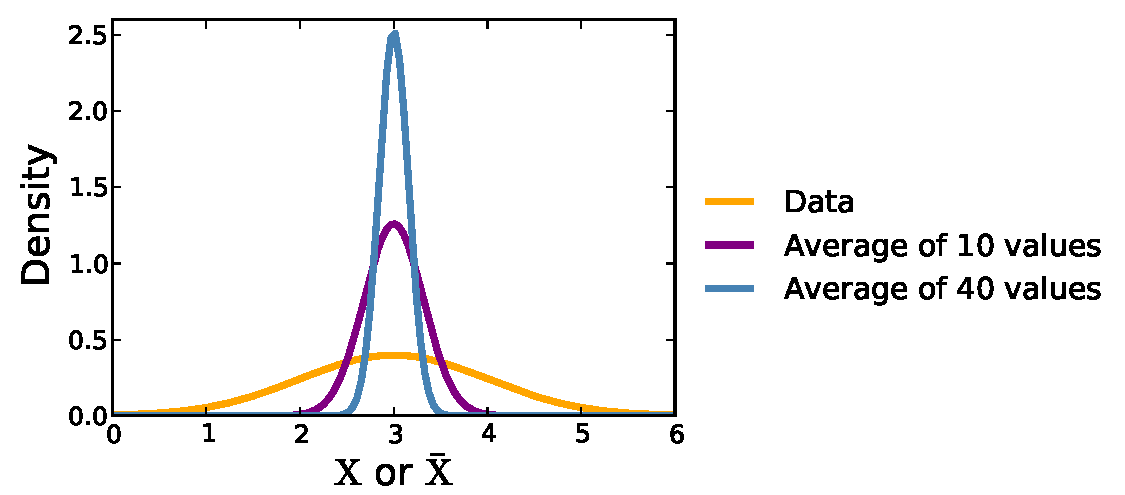
\includegraphics{045.pdf}}
%\end{center}
%
%\end{frame}
%
%
%
%
%\begin{frame}
%\frametitle{Sampling behavior of the sample mean}
%
%The following graphs show sampling distributions for $\bar{X}$ for a
%certain population of $X_i$ values.  The value of $\mu = EX_i$ is
%zero.
%
%\begin{center}
%\begin{tabular}{ccc}
%\scalebox{0.4}{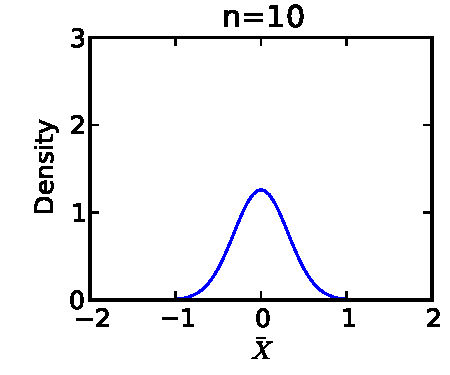
\includegraphics{008_0.pdf}} &
%\scalebox{0.4}{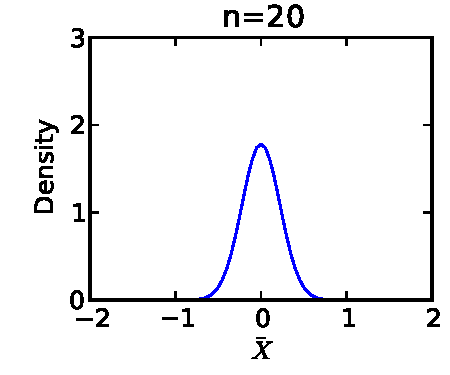
\includegraphics{008_1.pdf}} &
%\scalebox{0.4}{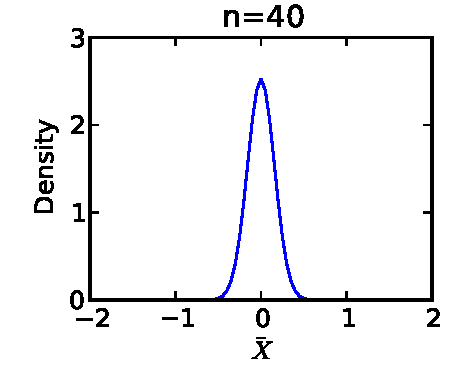
\includegraphics{008_2.pdf}}
%\end{tabular}
%\end{center}
%
%Note that this is for a particular distribution for $X_i$.  Different
%distributions will give different sampling distributions, but the
%reduction in scale as $n$ increases happens for many (but not all)
%distributions.
%
%\end{frame}
%

%%

%%%%%%%%%%%%%%%%%%%%%%%%%%%%%%%%%%%%%%%%%%%%%%%%%%%%%%%%%%%
\begin{frame}[fragile]\frametitle{Covariance and Correlation}
Both show association between two variables
\begin{itemize}
\item Positive: If one goes up, the other does too and vice versa.
\item Example: Height and weight
\item Not always, but tendency
\item Another example: Temperature and Ice-creame sales
\item Negative: Temperature and sale of woolen clothes
\end{itemize}
\end{frame}

%%%%%%%%%%%%%%%%%%%%%%%%%%%%%%%%%%%%%%%%%%%%%%%%%%%%%%%%%%%
\begin{frame}[fragile]\frametitle{Correlation}
\begin{itemize}
\item Correlation is a value standardized between -1 to 1
\item Relation between two variables is linear, 
\item Directly proportional in case of Positive Corr
\item Inversely proportional in case of Negative Corr
\item The value of corr is the factor of proportionality
\item No correlation, ie no dependence so value = 0
\end{itemize}
\end{frame}

%%%%%%%%%%%%%%%%%%%%%%%%%%%%%%%%%%%%%%%%%%%%%%%%%%%%%%%%%%%
\begin{frame}[fragile]\frametitle{Covariance and Correlation}
\begin{center}
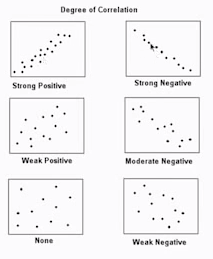
\includegraphics[width=0.6\linewidth,keepaspectratio]{corrplot}
\end{center}
\end{frame}

%%%%%%%%%%%%%%%%%%%%%%%%%%%%%%%%%%%%%%%%%%%%%%%%%%%%%%%%%%%
\begin{frame}[fragile]\frametitle{Covariance and Correlation}
The {\bf covariance} between $X$ and $Y$ is

$$
{\rm cov}(X,Y) \equiv E[(X-EX)(Y-EY)].
$$

\begin{center}
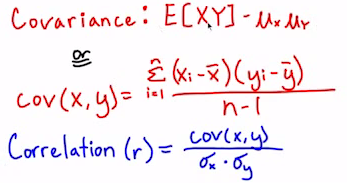
\includegraphics[width=0.6\linewidth,keepaspectratio]{corrcov}
\end{center}
\end{frame}


%%%%%%%%%%%%%%%%%%%%%%%%%%%%%%%%%%%%%%%%%%%%%%%%%%%
\begin{frame}
\frametitle{Covariance}
%
%Suppose we have a pair of random variables $X$ and $Y$ observed
%simultaneously.
%
%The {\bf covariance} between $X$ and $Y$ is
%
%$$
%{\rm cov}(X,Y) \equiv E[(X-EX)(Y-EY)].
%$$

Note the following two relationships:

\begin{itemize}

\item If $X>EX$ and $Y>EY$, or $X<EX$ and $Y<EY$, then $(X-EX)(Y-EY)>0$.

\item If $X>EX$ and $Y<EY$, or $X<EX$ and $Y>EY$, then $(X-EX)(Y-EY)<0$.

\end{itemize}

Thus, the covariance is positive if $X$ and $Y$ tend to be on the same
side of their respective mean values.

\end{frame}

%%%%%%%%%%%%%%%%%%%%%%%%%%%%%%%%%%%%%%%%%%%%%%%%%%%
\begin{frame}
\frametitle{Co-variance}

Here are two important properties of the co-variance:

\begin{itemize}

\item If $X$ or $Y$ is centered (i.e.\ has mean zero) then the
  covariance is simply ${\rm cov}(X,Y) = E[XY]$.

\item If $X$ and $Y$ are independent, their covariance is zero.

\end{itemize}

\end{frame}

%%%%%%%%%%%%%%%%%%%%%%%%%%%%%%%%%%%%%%%%%%%%%%%%%%%
\begin{frame}
\frametitle{Exercise: Co-variance}

Relation between Company Sales Value vs Marketing Spend
\begin{center}
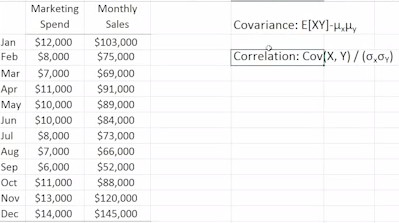
\includegraphics[width=0.8\linewidth,keepaspectratio]{covcorrex}
\end{center}
Put the values in excel and calculate.
\end{frame}

%%%%%%%%%%%%%%%%%%%%%%%%%%%%%%%%%%%%%%%%%%%%%%%%%%%
\begin{frame}
\frametitle{Exercise: Co-variance}

Plot the points (pairs x y)
\begin{center}
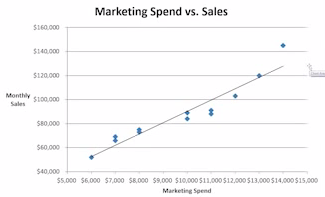
\includegraphics[width=0.5\linewidth,keepaspectratio]{covcorrplot}
\end{center}
Can we fit a line?
\end{frame}

%%%%%%%%%%%%%%%%%%%%%%%%%%%%%%%%%%%%%%%%%%%%%%%%%%%
\begin{frame}
\frametitle{Exercise: Covariance}
Expected value E[XY] is just mean of X*Y.
\begin{center}
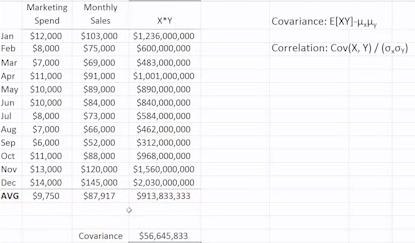
\includegraphics[width=0.65\linewidth,keepaspectratio]{covcorrex1}
\end{center}
\end{frame}

%%%%%%%%%%%%%%%%%%%%%%%%%%%%%%%%%%%%%%%%%%%%%%%%%%%
\begin{frame}
\frametitle{Exercise: Co-variance}
\begin{itemize}
\item Once co-variance value is ready, use it calculate Corr, with additional inputs of std deviations. 
\item It comes to 0.95. HIGH
\item Which is what plot also confirmed.
\end{itemize}
\end{frame}


%%
%%%%%%%%%%%%%%%%%%%%%%%%%%%%%%%%%%%%%%%%%%%%%%%%%%%%%
%%\begin{frame}
%%\frametitle{Properties of covariance}
%%
%%\begin{itemize}
%%
%%\item The variance of $X$ is the covariance of $X$ with itself: ${\rm
%%var}(X) = {\rm cov}(X,X)$.
%%
%%\item Covariance is symmetric: ${\rm cov}(A,B) = {\rm cov}(B,A)$.
%%
%%\item Covariance is \textcolor{purple}{bilinear}, which means that for
%%  random variables $A,B,C$ and a constant $k$:
%%
%%$$
%%\begin{array}{c}
%%{\rm cov}(A+B,C) = {\rm cov}(A,C) + {\rm cov}(B,C)\\
%%{\rm cov}(A,B+C) = {\rm cov}(A,B) + {\rm cov}(A,C)\\
%%{\rm cov}(kA,B) = {\rm cov}(A,kB) = k{\rm cov}(A,B)\\
%%\end{array}
%%$$
%%
%%\item The covariance between a random variable and a constant is
%%  zero: ${\rm cov}(A,k) = 0$, which also implies that ${\rm
%%    cov}(A,B+k) = {\rm cov}(A,B)$.
%%
%%\end{itemize}
%%
%%\end{frame}
%%
%%%%%%%%%%%%%%%%%%%%%%%%%%%%%%%%%%%%%%%%%%%%%%%%%%%%%
%%\begin{frame}
%%\frametitle{Properties of covariance}
%%
%%The following identities follow from the identities on the previous slide:
%%
%%$$ {\rm cov}(A+B, C+D) = {\rm cov}(A,C) + {\rm cov}(A,D) + {\rm
%%cov}(B,C) + {\rm cov}(B,D)
%%$$
%%
%%$$ {\rm cov}(k_1A, k_2B) = k_1k_2{\rm cov}(A,B)
%%$$
%%
%%\end{frame}
%%
%%%%%%%%%%%%%%%%%%%%%%%%%%%%%%%%%%%%%%%%%%%%%%%%%%%%%
%%\begin{frame}
%%\frametitle{Calculating the covariance}
%%
%%Suppose we have the following joint distribution:
%%
%%\begin{center}
%%\begin{tabular}{rrrrr}
%%    &   & \multicolumn{3}{c}{$X$}\\
%%    &   & -1 & 0 & 1 \\\hline
%%    &-1 & 0.1 & 0.0 & 0.2\\
%%$Y$ & 0 & 0.1 & 0.3 & 0.0 \\
%%    & 1 & 0.0 & 0.2 & 0.1
%%\end{tabular}
%%\end{center}
%%
%%The marginal means are:
%%
%%$$
%%EX = -1\cdot 0.2 + 0\cdot 0.5 + 1\cdot 0.3 = 0.1
%%$$
%%
%%$$
%%EY = -1\cdot 0.3 + 0\cdot 0.4 + 1\cdot 0.3 = 0
%%$$
%%
%%\end{frame}
%%
%%%%%%%%%%%%%%%%%%%%%%%%%%%%%%%%%%%%%%%%%%%%%%%%%%%%%
%%\begin{frame}
%%\frametitle{Calculating the covariance}
%%
%%We can make a table of values of $(X-EX)\cdot(Y-EY)$:
%%
%%\begin{center}
%%\begin{tabular}{rrccc}
%%    &   & \multicolumn{3}{c}{$X$}\\
%%    &   & -1 & 0 & 1 \\\hline
%%    &-1 & $-1.1\cdot -1 = 1.1$ & $-0.1\cdot -1 = 0.1$ & $0.9\cdot -1 = -0.9$ \\
%%$Y$ & 0 & $-1.1\cdot 0 = 0$ & $-0.1\cdot 0 = 0$ & $0.9\cdot 0 = 0$ \\
%%    & 1 & $-1.1\cdot 1 = -1.1$ & $-0.1\cdot 1 = -0.1$ & $0.9\cdot 1 = 0.9$ \\
%%\hline
%%\end{tabular}
%%\end{center}
%%
%%The covariance is
%%
%%\begin{eqnarray*}
%%{\rm cov}(X,Y) &=& 1.1\cdot 0.1 + 0.1\cdot 0 - 0.9\cdot 0.2 + 0\cdot
%%0.1 + 0\cdot 0.3 +\\&&\;\;\; 0\cdot 0 -1.1\cdot 0 - 0.1\cdot 0.2 +
%%0.9\cdot 0.1\\ &=& 0.
%%\end{eqnarray*}
%%
%%
%%\end{frame}
%%
%%%%%%%%%%%%%%%%%%%%%%%%%%%%%%%%%%%%%%%%%%%%%%%%%%%%%
%%\begin{frame}
%%\frametitle{Estimating variances and covariances}
%%
%%Suppose we have data $X_1, \ldots, X_n$.  The variance of the
%%distribution of the $X_i$ can be estimated using the
%%\textcolor{purple}{sample variance}
%%
%%$$
%%\frac{1}{n-1}\sum_{i=1}^n (X_i-\bar{X})^2.
%%$$
%%
%%If we have paired data $(X_1,Y_1), \ldots, (X_n,Y_n)$, the covariance
%%between $X$ and $Y$ can be estimated by the \textcolor{purple}{sample
%%  covariance}
%%
%%$$
%%\frac{1}{n-1}\sum_{i=1}^n (X_i-\bar{X})(Y_i-\bar{Y}).
%%$$
%%
%%\end{frame}
%%
%%
%%%%%%%%%%%%%%%%%%%%%%%%%%%%%%%%%%%%%%%%%%%%%%%%%%%%%
%%\begin{frame}
%%\frametitle{Correlation}
%%
%%The \textcolor{purple}{correlation coefficient} between $X$ and $Y$ is
%%
%%$$
%%r \equiv \frac{{\rm cov}(X,Y)}{{\rm SD}(X)\cdot {\rm SD}(Y)}.
%%$$
%%
%%This is sometimes called the ``Pearson correlation coefficient.''
%%
%%
%%It is a fact that $-1 \le r \le 1$, and that $|r|=1$ only if $X$ and
%%$Y$ are linearly related.
%%
%%Since $r$ has the same sign as the covariance, it also tends to be
%%positive in situations where $X$ and $Y$ tend to be on the same side of
%%their respective mean values.
%%
%%If ${\rm SD}(X)=0$ or ${\rm SD}(Y)=0$, $r$ is undefined.
%%
%%\end{frame}
%%
%%%%%%%%%%%%%%%%%%%%%%%%%%%%%%%%%%%%%%%%%%%%%%%%%%%%%
%%\begin{frame}
%%\frametitle{Correlation}
%%
%%The main application of the correlation coefficient is to measure the
%%degree of linear association between $X$ and $Y$.  The following plots
%%illustrate what is captured by the correlation coefficient.
%%
%%
%%\begin{center}
%%\begin{tabular}{cc}
%%\scalebox{0.5}{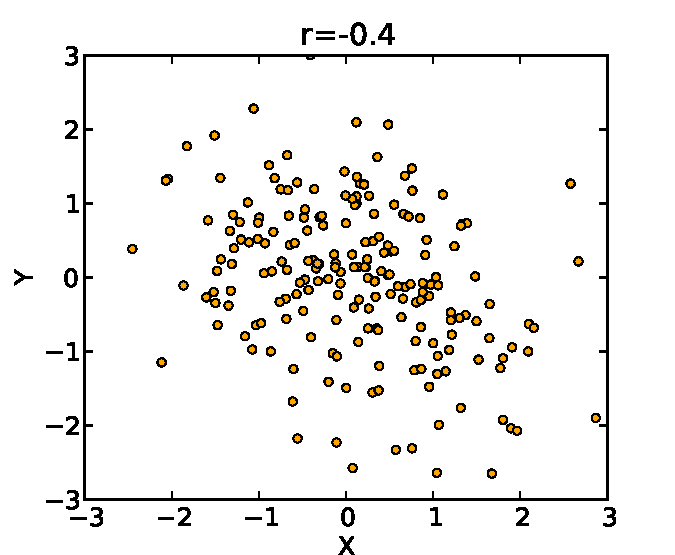
\includegraphics{022_0.pdf}} &
%%\scalebox{0.5}{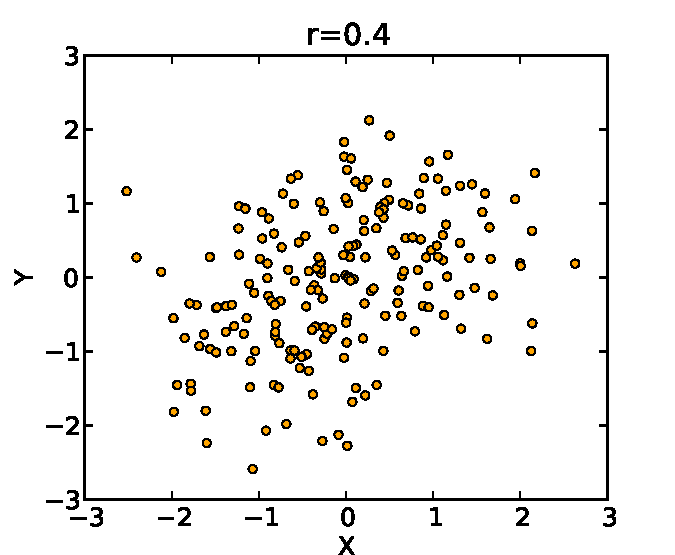
\includegraphics{022_1.pdf}}
%%\end{tabular}
%%\end{center}
%%
%%\end{frame}
%%
%%%%%%%%%%%%%%%%%%%%%%%%%%%%%%%%%%%%%%%%%%%%%%%%%%%%%
%%\begin{frame}
%%\frametitle{Correlation}
%%
%%\begin{center}
%%\begin{tabular}{cc}
%%\scalebox{0.5}{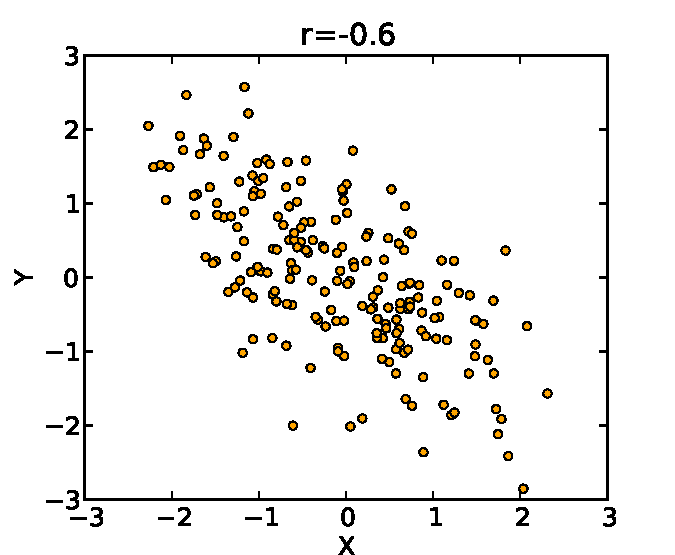
\includegraphics{022_2.pdf}} &
%%\scalebox{0.5}{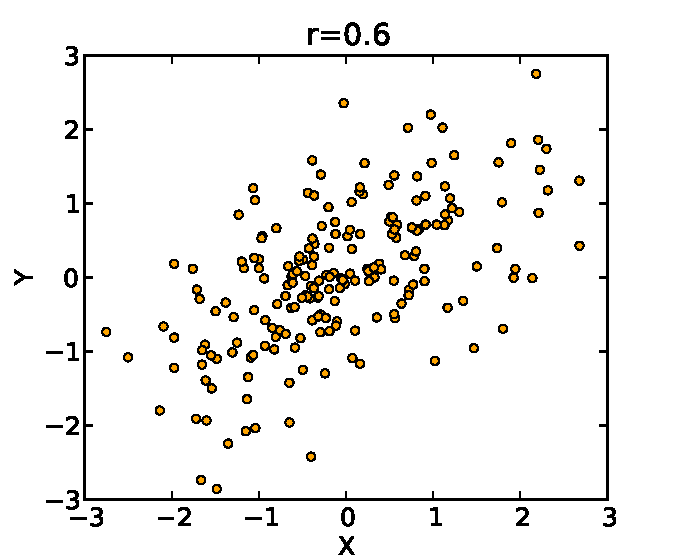
\includegraphics{022_3.pdf}}
%%\end{tabular}
%%\end{center}
%%
%%\end{frame}
%%
%%%%%%%%%%%%%%%%%%%%%%%%%%%%%%%%%%%%%%%%%%%%%%%%%%%%%
%%\begin{frame}
%%\frametitle{Correlation}
%%
%%\begin{center}
%%\begin{tabular}{cc}
%%\scalebox{0.5}{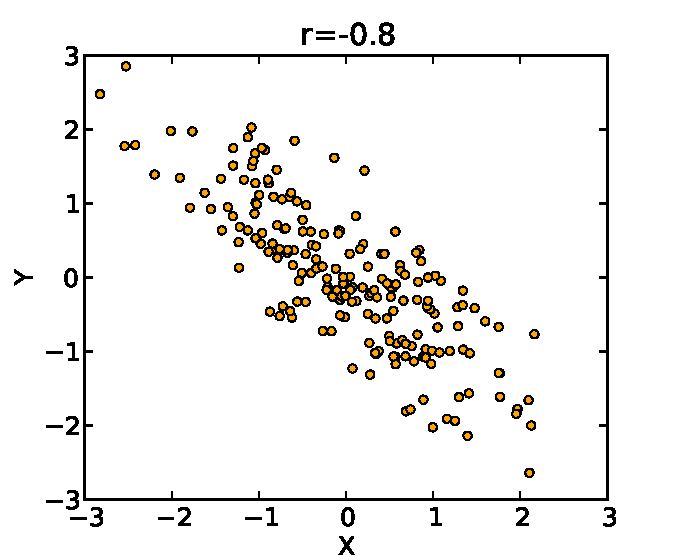
\includegraphics{022_4.pdf}} &
%%\scalebox{0.5}{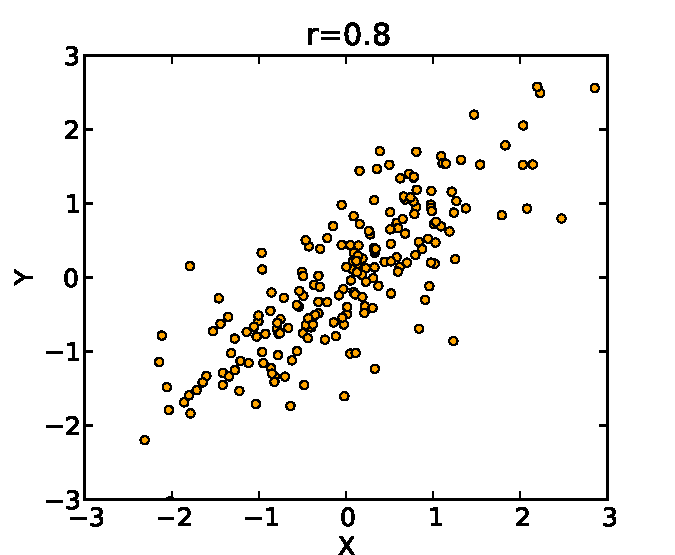
\includegraphics{022_5.pdf}}
%%\end{tabular}
%%\end{center}
%%
%%\end{frame}
%%
%%%%%%%%%%%%%%%%%%%%%%%%%%%%%%%%%%%%%%%%%%%%%%%%%%%%%
%%\begin{frame}
%%\frametitle{Correlation}
%%
%%\begin{center}
%%\begin{tabular}{cc}
%%\scalebox{0.5}{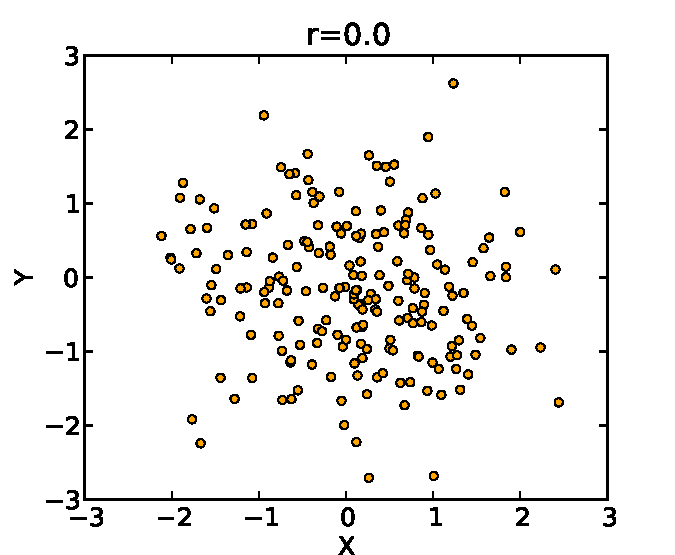
\includegraphics{022_6.pdf}} &
%%\scalebox{0.5}{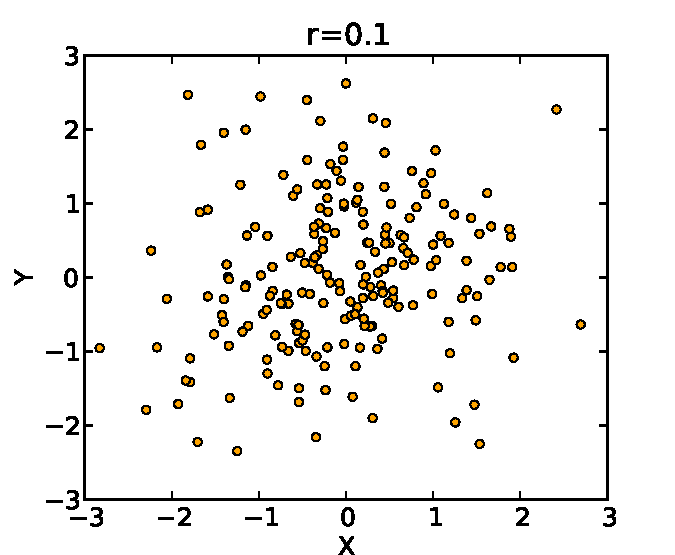
\includegraphics{022_7.pdf}}
%%\end{tabular}
%%\end{center}
%%
%%\end{frame}
%%
%%%%%%%%%%%%%%%%%%%%%%%%%%%%%%%%%%%%%%%%%%%%%%%%%%%%%
%%\begin{frame}
%%\frametitle{Correlation}
%%
%%Correlation coefficients are mainly useful for picking up a linear
%%trend.  The plot on the left shows a strong relationship between $X$
%%and $Y$, but the correlation is nearly zero.  The plot on the right is
%%not linear, but since it is non-decreasing it still gives a
%%substantial correlation.
%%
%%\begin{center}
%%\begin{tabular}{cc}
%%\scalebox{0.5}{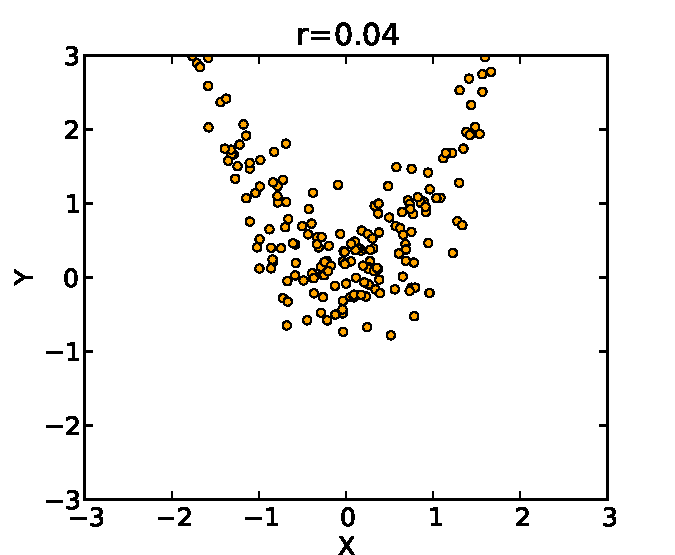
\includegraphics{023.pdf}} &
%%\scalebox{0.5}{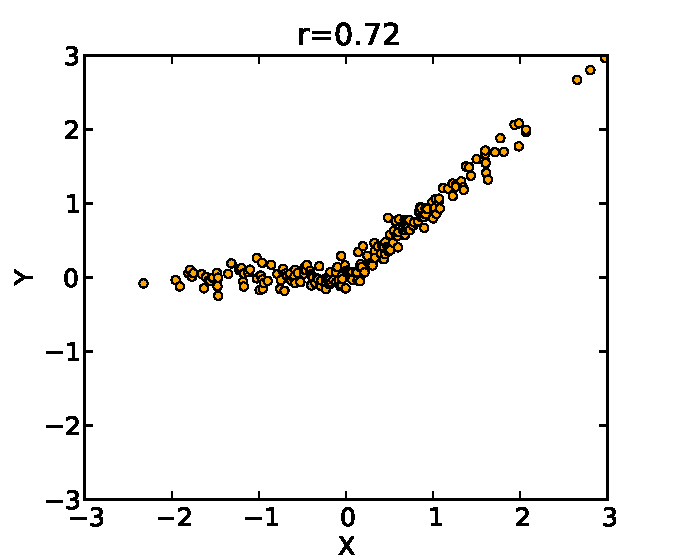
\includegraphics{024.pdf}}
%%\end{tabular}
%%\end{center}
%%
%%\end{frame}
%%
%%%%%%%%%%%%%%%%%%%%%%%%%%%%%%%%%%%%%%%%%%%%%%%%%%%%%
%%\begin{frame}
%%\frametitle{Covariance matrices}
%%
%%Suppose we have several dependent random variables $Y_1, Y_2, \ldots,
%%Y_m$.  We can calculate the covariance ${\rm cov}(Y_i, Y_j)$ between
%%any two of them.
%%
%%The \textcolor{purple}{covariance matrix} is a matrix whose $i,j$
%%element is ${\rm cov}(Y_i,Y_j)$.
%%
%%For example, with $m=3$ random variables we might have
%%
%%
%%$$ \left(\begin{array}{ccc} {\rm var}(Y_1) & {\rm cov}(Y_1,Y_2) & {\rm
%%cov}(Y_1,Y_3)\\ {\rm cov}(Y_2,Y_1) & {\rm var}(Y_2) & {\rm
%%cov}(Y_2,Y_3)\\ {\rm cov}(Y_3,Y_1) & {\rm cov}(Y_3,Y_2) & {\rm
%%var}(Y_3)\end{array}\right) = \left(\begin{array}{ccc} 3 & 3 & 2\\ 3 &
%%4 & 3\\ 2 & 3 & 5\end{array}\right)
%%$$
%%
%%\end{frame}


%%%%%%%%%%%%%%%%%%%%%%%%%%%%%%%%%%%%%%%%%%%%%%%%%%%%%%%%%%
\begin{frame}[fragile]\frametitle{}
\begin{center}
{\Large Example}
\end{center}
\end{frame}

%%%%%%%%%%%%%%%%%%%%%%%%%%%%%%%%%%%%%%%%%%%%%%%%%%%%%%%%%%
\begin{frame}
\frametitle{Example}
You purchase a raffle (Lottery) ticket to help out a the high school football team. The raffle ticket costs \$20 and 1,500 tickets are sold. One of them will be drawn and the winner receives \$1,000. Compute the expected value for this raffle.
\end{frame}


%%%%%%%%%%%%%%%%%%%%%%%%%%%%%%%%%%%%%%%%%%%%%%%%%%%%%%%%%%
\begin{frame}
\frametitle{Example}
\begin{center}
\begin{tabular}{|c|c|}
\hline
Outcome	&Probability of outcome\\
\hline
&\\
	  & \\
&\\
\hline
&\\
	& \\
&\\
\hline
\end{tabular} 
\end{center}
\end{frame}


%%%%%%%%%%%%%%%%%%%%%%%%%%%%%%%%%%%%%%%%%%%%%%%%%%%%%%%%%%
\begin{frame}
\frametitle{Example}
\begin{center}
\begin{tabular}{|c|c|}
\hline
Outcome	&Probability of outcome\\
\hline
&\\
\$980	  & \\
&\\
\hline
&\\
	& \\
&\\
\hline
\end{tabular} 
\end{center}
\end{frame}

%%%%%%%%%%%%%%%%%%%%%%%%%%%%%%%%%%%%%%%%%%%%%%%%%%%%%%%%%%
\begin{frame}
\frametitle{Example}

\begin{center}
\begin{tabular}{|c|c|}
\hline
Outcome	&Probability of outcome\\
\hline
&\\
\$980	  & \\
&\\
\hline
&\\
-\$20	& \\
&\\
\hline
\end{tabular} 
\end{center}
\end{frame}

%%%%%%%%%%%%%%%%%%%%%%%%%%%%%%%%%%%%%%%%%%%%%%%%%%%%%%%%%%
\begin{frame}
\frametitle{Example}
\begin{center}
\begin{tabular}{|c|c|}
\hline
Outcome	&Probability of outcome\\
\hline
&\\
\$980	  & $\frac{1}{1,500}$ \\
&\\
\hline
&\\
-\$20	& \\
&\\
\hline
\end{tabular} 
\end{center}
\end{frame}

%%%%%%%%%%%%%%%%%%%%%%%%%%%%%%%%%%%%%%%%%%%%%%%%%%%%%%%%%%
\begin{frame}
\frametitle{Example}
\begin{center}
\begin{tabular}{|c|c|}
\hline
Outcome	&Probability of outcome\\
\hline
&\\
\$980	  & $\frac{1}{1,500}$ \\
&\\
\hline
&\\
-\$20	& $\frac{1,499}{1,500}$ \\
&\\
\hline
\end{tabular} 
\end{center}

\begin{equation*}
\$980\cdot \frac{1}{1500}-\$20\cdot \frac{1499}{1500} =  -\$19.33
\end{equation*}
\end{frame}

%%%%%%%%%%%%%%%%%%%%%%%%%%%%%%%%%%%%%%%%%%%%%%%%%%%%%%%%%%
\begin{frame}[fragile]\frametitle{}
\begin{center}
{\Large Example}
\end{center}
\end{frame}

%%%%%%%%%%%%%%%%%%%%%%%%%%%%%%%%%%%%%%%%%%%%%%%%%%%%%%%%%%
\begin{frame}
\frametitle{Example}
A game involves rolling two dice.  If the sum is 12, you win \$10, otherwise if the sum is greater than 8, you win \$5.  It costs \$2 to play.  What is the expected value?  Should you play?
\end{frame}

%%%%%%%%%%%%%%%%%%%%%%%%%%%%%%%%%%%%%%%%%%%%%%%%%%%%%%%%%%
\begin{frame}
\frametitle{Example}
\begin{center}
\begin{tabular}{|c|c|}
\hline
Outcome	&Probability of outcome\\
\hline
&\\
  &  \\
&\\
\hline
&\\
&  \\
&\\
\hline
&\\
&\\
&\\
\hline
\end{tabular} 
\end{center}
\end{frame}

%%%%%%%%%%%%%%%%%%%%%%%%%%%%%%%%%%%%%%%%%%%%%%%%%%%%%%%%%%
\begin{frame}
\frametitle{Example}
Outcome is prize minus cost (\$2). Those who do not have any prize their outcome is 0 minus \$2, ie -\$2.
\begin{center}
\begin{tabular}{|c|c|}
\hline
Outcome	&Probability of outcome\\
\hline
&\\
\$8  &  \\
&\\
\hline
&\\
&  \\
&\\
\hline
&\\
&\\
&\\
\hline
\end{tabular} 
\end{center}
\end{frame}

%%%%%%%%%%%%%%%%%%%%%%%%%%%%%%%%%%%%%%%%%%%%%%%%%%%%%%%%%%
\begin{frame}
\frametitle{Example}
\begin{center}
\begin{tabular}{|c|c|}
\hline
Outcome	&Probability of outcome\\
\hline
&\\
\$8  &  \\
&\\
\hline
&\\
\$3&  \\
&\\
\hline
&\\
&\\
&\\
\hline
\end{tabular} 
\end{center}
\end{frame}

%%%%%%%%%%%%%%%%%%%%%%%%%%%%%%%%%%%%%%%%%%%%%%%%%%%%%%%%%%
\begin{frame}
\frametitle{Example}
\begin{center}
\begin{tabular}{|c|c|}
\hline
Outcome	&Probability of outcome\\
\hline
&\\
\$8  &  \\
&\\
\hline
&\\
\$3&  \\
&\\
\hline
&\\
-\$2&\\
&\\
\hline
\end{tabular} 
\end{center}
\end{frame}

%%%%%%%%%%%%%%%%%%%%%%%%%%%%%%%%%%%%%%%%%%%%%%%%%%%%%%%%%%
\begin{frame}
\frametitle{Example}
\begin{center}
\begin{tabular}{|c|c|}
\hline
Outcome	&Probability of outcome\\
\hline
&\\
\$8  & $\frac{1}{36}$ \\
&\\
\hline
&\\
\$3&  \\
&\\
\hline
&\\
-\$2&\\
&\\
\hline
\end{tabular} 
\end{center}
\end{frame}

%%%%%%%%%%%%%%%%%%%%%%%%%%%%%%%%%%%%%%%%%%%%%%%%%%%%%%%%%%
\begin{frame}
\frametitle{Example}

\begin{center}
\begin{tabular}{|c|c|}
\hline
Outcome	&Probability of outcome\\
\hline
&\\
\$8  & $\frac{1}{36}$ \\
&\\
\hline
&\\
\$3& $\frac{9}{36}$ \\
&\\
\hline
&\\
-\$2&\\
&\\
\hline
\end{tabular} 
\end{center}
\end{frame}

%%%%%%%%%%%%%%%%%%%%%%%%%%%%%%%%%%%%%%%%%%%%%%%%%%%%%%%%%%
\begin{frame}
\frametitle{Example}
\begin{center}
\begin{tabular}{|c|c|}
\hline
Outcome	&Probability of outcome\\
\hline
&\\
\$8  & $\frac{1}{36}$ \\
&\\
\hline
&\\
\$3& $\frac{9}{36}$ \\
&\\
\hline
&\\
-\$2& $\frac{26}{36}$\\
&\\
\hline
\end{tabular} 
\end{center}
\end{frame}

%%%%%%%%%%%%%%%%%%%%%%%%%%%%%%%%%%%%%%%%%%%%%%%%%%%%%%%%%%
\begin{frame}
\frametitle{Example}

\begin{equation*}
\$8\cdot \frac{1}{36} + \$3\cdot \frac{9}{36} -\$2\cdot \frac{26}{36}=-\$0.47
\end{equation*}

The expected value : the mean profit per ticket is the value we expect to get, on average, from each ticket.

For this game, each time you buy a ticket you lose an average of $0.47. Of course, you never actually lose $0.47: you either lose $2 or gain $8 or $3 (-$0.47 is just an average).
\end{frame}



%%%%%%%%%%%%%%%%%%%%%%%%%%%%%%%%%%%%%%%%%%%%%%%%%%%%%%%%%%
\begin{frame}
\frametitle{Example}
What if cost is \$1 to play?  What is the expected value?  Play?

\begin{center}
\begin{tabular}{|c|c|}
\hline
Outcome	&Probability of outcome\\
\hline
&\\
\$9  & $\frac{1}{36}$ \\
&\\
\hline
&\\
\$4& $\frac{9}{36}$ \\
&\\
\hline
&\\
-\$1& $\frac{26}{36}$\\
&\\
\hline
\end{tabular} 
\end{center}
\end{frame}

%%%%%%%%%%%%%%%%%%%%%%%%%%%%%%%%%%%%%%%%%%%%%%%%%%%%%%%%%%
\begin{frame}
\frametitle{Example}
\begin{equation*}
\$9\cdot \frac{1}{36} + \$4\cdot \frac{9}{36} -\$1\cdot \frac{26}{36}= \$0.53
\end{equation*}
POSITIVE expected value, means?
\end{frame}

